\documentclass[11pt,spanish]{beamer}
\usepackage{mathpazo}
\usepackage{tgheros}
\renewcommand{\familydefault}{\sfdefault}
\usepackage[T1]{fontenc}
\usepackage[utf8]{inputenc}
\usepackage{babel}
\usepackage{amsmath}
\usepackage{amssymb}
\usepackage{array}
\usepackage{tikz}
\usetikzlibrary{automata,arrows.meta,calc,positioning,shapes.geometric}

\definecolor{Guinda}{rgb}{0.49,0.05,0.12}
\definecolor{Rojo}{rgb}{0.8,0,0}
\definecolor{indiagreen}{rgb}{0.07,0.53,0.03}
\definecolor{anti-flashwhite}{rgb}{0.95,0.95,0.96}
\definecolor{pastelblue}{rgb}{0.78,0.87,0.96}
\definecolor{pastelgreen}{rgb}{0.82,0.92,0.78}
\definecolor{pastelpeach}{rgb}{0.98,0.84,0.72}
\definecolor{pastelrose}{rgb}{0.96,0.78,0.84}
\definecolor{pastelviolet}{rgb}{0.86,0.80,0.96}
\definecolor{pastelyellow}{rgb}{0.98,0.93,0.70}

\usecolortheme[named=indiagreen]{structure}
\usetheme{Boadilla}
\usefonttheme{structurebold}
\setbeamertemplate{itemize items}[default]
\setbeamertemplate{enumerate items}[default]
\setbeamertemplate{navigation symbols}{}
\setbeamercolor{block title}{fg=white,bg=indiagreen!85!black}
\setbeamercolor{block body}{fg=black,bg=pastelgreen!45!white}

\hypersetup{hidelinks}
\addto\shorthandsspanish{\spanishdeactivate{~<>.}}
\deactivatequoting
\newcommand{\term}[1]{\textbf{\textcolor{indiagreen!80!black}{#1}}}
\newcommand{\actividad}[1]{\textbf{\textcolor{Rojo}{#1}}}
\newcolumntype{L}[1]{>{\raggedright\arraybackslash}p{#1}}

\hyphenpenalty=9000
\exhyphenpenalty=9000
\emergencystretch=2em

\tikzset{
  idea/.style={
    rounded corners=3pt,
    draw=indiagreen!70!black,
    fill=pastelgreen,
    align=center,
    inner sep=7pt,
    font=\small
  },
  bloque/.style={
    rounded corners=3pt,
    draw=black!35,
    fill=pastelblue,
    align=center,
    text width=2.8cm,
    minimum height=1.05cm,
    inner sep=5pt,
    font=\small
  },
  mini/.style={
    rounded corners=3pt,
    draw=black!35,
    fill=anti-flashwhite,
    align=center,
    text width=2.35cm,
    minimum height=.85cm,
    inner sep=4pt,
    font=\scriptsize
  },
  paso/.style={
    rounded corners=3pt,
    draw=indiagreen!70!black,
    fill=pastelgreen,
    align=center,
    text width=2.05cm,
    minimum height=.95cm,
    inner sep=4pt,
    font=\scriptsize
  },
  arrow/.style={
    -{Stealth[length=2.5mm]},
    thick,
    indiagreen!80!black
  }
}

\title[PDS]{\textbf{Expresiones regulares y autómatas}}
\subtitle{Repaso de la Nota 04 y trabajo con el Cuadernillo de ejercicios 03%
\ifkahoot\else\\[0.35em]\textit{Versión sin kahoot}\fi}
\author[Soto Romero y Reyes Cabello]{Manuel Soto Romero \and Araceli Liliana Reyes Cabello}
\institute[UACM]{Colegio de Ciencia y Tecnología, UACM}
\date{Semestre 2026-2}

\begin{document}

\begin{frame}
\titlepage
\end{frame}

\ifkahoot
\begin{frame}{Iniciamos con \textsc{Kahoot}}
\vfill

\begin{center}
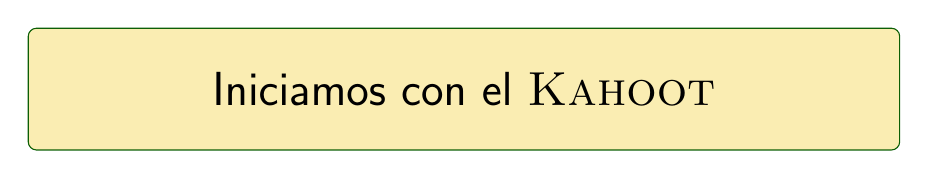
\begin{tikzpicture}
\node[
  idea,
  fill=pastelyellow,
  text width=.82\textwidth,
  inner sep=16pt,
  font=\LARGE
]
{Iniciamos con el \textsc{Kahoot}};
\end{tikzpicture}
\end{center}

\vfill
\end{frame}
\fi

\begin{frame}{Ruta de trabajo}
\vfill

\begin{center}
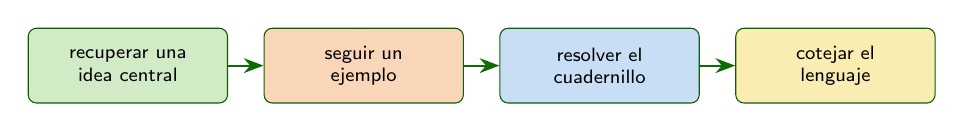
\begin{tikzpicture}[node distance=.45cm]
\node[paso,fill=pastelgreen,text width=2.25cm] (a) {recuperar una\\idea central};
\node[paso,fill=pastelpeach,right=of a,text width=2.25cm] (b) {seguir un\\ejemplo};
\node[paso,fill=pastelblue,right=of b,text width=2.25cm] (c) {resolver el\\cuadernillo};
\node[paso,fill=pastelyellow,right=of c,text width=2.25cm] (d) {cotejar el\\lenguaje};
\draw[arrow] (a) -- (b);
\draw[arrow] (b) -- (c);
\draw[arrow] (c) -- (d);
\end{tikzpicture}
\end{center}

\bigskip

\begin{block}{Durante la sesión}
Alternaremos el repaso de la Nota 04 con los ejercicios del \term{Cuadernillo de ejercicios 03}.
\end{block}

\begin{center}
\small En cada transformación preguntaremos: ¿cambió la representación o cambió el lenguaje?
\end{center}

\vfill
\end{frame}

\begin{frame}{Del patrón a un reconocedor}
\vfill

\begin{center}
\resizebox{.97\textwidth}{!}{%
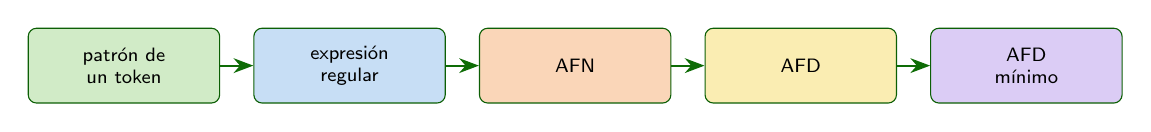
\begin{tikzpicture}[node distance=.42cm]
\node[paso,fill=pastelgreen,text width=2.15cm] (a) {patrón de\\un token};
\node[paso,fill=pastelblue,right=of a,text width=2.15cm] (b) {expresión\\regular};
\node[paso,fill=pastelpeach,right=of b,text width=2.15cm] (c) {AFN};
\node[paso,fill=pastelyellow,right=of c,text width=2.15cm] (d) {AFD};
\node[paso,fill=pastelviolet,right=of d,text width=2.15cm] (e) {AFD\\mínimo};
\draw[arrow] (a) -- (b);
\draw[arrow] (b) -- (c);
\draw[arrow] (c) -- (d);
\draw[arrow] (d) -- (e);
\end{tikzpicture}%
}
\end{center}

\bigskip

\begin{columns}[T,onlytextwidth]
\begin{column}{.48\textwidth}
\begin{block}{Especificar}
\small Describe cuáles cadenas pertenecen a una categoría léxica.
\end{block}
\end{column}
\begin{column}{.48\textwidth}
\begin{block}{Reconocer}
\small Recibe una cadena y decide si pertenece al lenguaje especificado.
\end{block}
\end{column}
\end{columns}

\bigskip
\begin{center}
\term{Las conversiones cambian la representación, pero conservan el lenguaje.}
\end{center}

\vfill
\end{frame}

\begin{frame}{Alfabeto, cadena y lenguaje}
\vfill

\begin{columns}[T,onlytextwidth]
\begin{column}{.30\textwidth}
\begin{block}{Alfabeto \(\Sigma\)}
\small Conjunto finito de símbolos.
\end{block}
\end{column}
\begin{column}{.30\textwidth}
\begin{block}{Cadena}
\small Secuencia finita de símbolos; \(\varepsilon\) es la cadena vacía.
\end{block}
\end{column}
\begin{column}{.30\textwidth}
\begin{block}{Lenguaje}
\small Conjunto de cadenas formadas sobre un alfabeto.
\end{block}
\end{column}
\end{columns}

\bigskip

\begin{center}
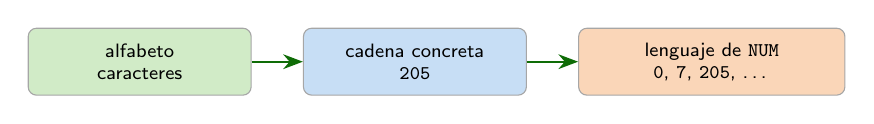
\begin{tikzpicture}[node distance=.65cm]
\node[mini,fill=pastelgreen,text width=2.55cm] (a) {alfabeto\\caracteres};
\node[mini,fill=pastelblue,right=of a,text width=2.55cm] (b) {cadena concreta\\\texttt{205}};
\node[mini,fill=pastelpeach,right=of b,text width=3.1cm] (c) {lenguaje de \texttt{NUM}\\\texttt{0}, \texttt{7}, \texttt{205}, \ldots};
\draw[arrow] (a) -- (b);
\draw[arrow] (b) -- (c);
\end{tikzpicture}
\end{center}

\bigskip
\begin{center}
\small \texttt{205} es una cadena del lenguaje de \texttt{NUM}; no es el lenguaje completo.
\end{center}

\vfill
\end{frame}

\begin{frame}{Operaciones de las expresiones regulares}
\vfill

\begin{center}
\small
\renewcommand{\arraystretch}{1.3}
\begin{tabular}{|L{.20\textwidth}|L{.18\textwidth}|L{.50\textwidth}|}
\hline
\textbf{Operación} & \textbf{Notación} & \textbf{Qué cadenas describe} \tabularnewline
\hline
Unión & \(r\mid s\) & Las que pertenecen a \(L(r)\), a \(L(s)\) o a ambos. \tabularnewline
\hline
Concatenación & \(rs\) & Las formadas al unir una cadena de \(L(r)\) con una de \(L(s)\). \tabularnewline
\hline
Cerradura & \(r^{*}\) & Cero o más repeticiones; siempre incluye \(\varepsilon\). \tabularnewline
\hline
Repetición positiva & \(r^{+}=rr^{*}\) & Una o más repeticiones; no incluye \(\varepsilon\) por sí sola. \tabularnewline
\hline
\end{tabular}
\end{center}

\bigskip
\begin{block}{Precedencia}
\centering
cerradura \(>\) concatenación \(>\) unión
\end{block}

\vfill
\end{frame}

\begin{frame}{Leamos el lenguaje antes de probar cadenas}
\vfill

\begin{center}
\small
\renewcommand{\arraystretch}{1.22}
\begin{tabular}{|L{.20\textwidth}|L{.67\textwidth}|}
\hline
\textbf{Expresión} & \textbf{Lenguaje denotado} \tabularnewline
\hline
\(a\mid b\) & \(\{a,b\}\). \tabularnewline
\hline
\(ab\) & Sólo la cadena \(ab\). \tabularnewline
\hline
\(a^{*}\) & \(\{\varepsilon,a,aa,aaa,\ldots\}\). \tabularnewline
\hline
\((a\mid b)^{*}\) & Todas las cadenas finitas sobre \(\{a,b\}\), incluida \(\varepsilon\). \tabularnewline
\hline
\(a(a\mid b)^{*}\) & Cadenas no vacías sobre \(\{a,b\}\) cuyo primer símbolo es \(a\). \tabularnewline
\hline
\end{tabular}
\end{center}

\bigskip
\begin{center}
\term{Pregunta de control: ¿qué exige la expresión y qué parte puede quedar vacía?}
\end{center}

\vfill
\end{frame}

\begin{frame}{Trabajo con el cuadernillo}
\vfill

\begin{center}
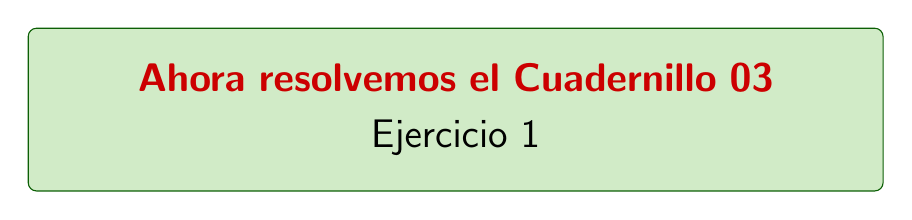
\begin{tikzpicture}
\node[idea,fill=pastelgreen,text width=.82\textwidth,inner sep=13pt,font=\Large]
{\actividad{Ahora resolvemos el Cuadernillo 03}\\[2pt]
Ejercicio 1};
\end{tikzpicture}
\end{center}

\bigskip
\begin{itemize}
\item \textbf{Ejercicio 1:} cotejar cadenas con varias expresiones regulares.
\item Al justificar, identifica qué operación obliga a consumir símbolos y cuál permite \(\varepsilon\).
\end{itemize}

\vfill
\end{frame}

\begin{frame}{Patrones variables del IMP básico}
\vfill

\[
\begin{aligned}
\mathit{letra}  & = \texttt{[A-Za-z]},\\
\mathit{digito} & = \texttt{[0-9]},\\
\mathit{LOC}    & = \mathit{letra}^{+}\mathit{digito}^{*},\\
\mathit{NUM}    & = \mathit{digito}^{+}.
\end{aligned}
\]

\begin{center}
\small
\renewcommand{\arraystretch}{1.2}
\begin{tabular}{|c|L{.25\textwidth}|L{.31\textwidth}|}
\hline
\textbf{Token} & \textbf{Sí satisface} & \textbf{No satisface} \tabularnewline
\hline
\texttt{LOC} & \texttt{x}, \texttt{total}, \texttt{x20} & \texttt{20x}, \texttt{x2y}, \texttt{x\_1} \tabularnewline
\hline
\texttt{NUM} & \texttt{0}, \texttt{25}, \texttt{2048} & \(\varepsilon\), \texttt{2x}, \texttt{-5} \tabularnewline
\hline
\end{tabular}
\end{center}

\vfill
\end{frame}

\begin{frame}{Cómo leer \texttt{LOC} y \texttt{NUM}}
\vfill

\begin{center}
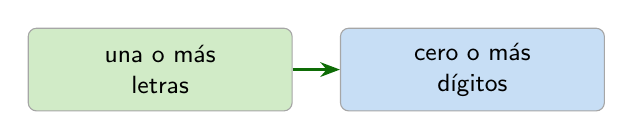
\begin{tikzpicture}[node distance=.6cm]
\node[bloque,fill=pastelgreen,text width=3cm] (a) {una o más\\letras};
\node[bloque,fill=pastelblue,right=of a,text width=3cm] (b) {cero o más\\dígitos};
\draw[arrow] (a) -- (b);
\end{tikzpicture}
\end{center}

\bigskip

\begin{itemize}
\item En \texttt{x2y}, una letra aparece después de comenzar la parte de dígitos.
\item En \texttt{20x}, falta la parte inicial de una o más letras.
\item En \texttt{-5}, el signo no es un dígito: se reconocería como \texttt{MINUS} seguido de \texttt{NUM(5)}.
\item \texttt{while} satisface \texttt{LOC} y también es un lexema fijo de \texttt{WHILE}; la coordinación de reglas pertenece al tema 2.3.
\end{itemize}

\vfill
\end{frame}

\begin{frame}{Trabajo con el cuadernillo}
\vfill

\begin{center}
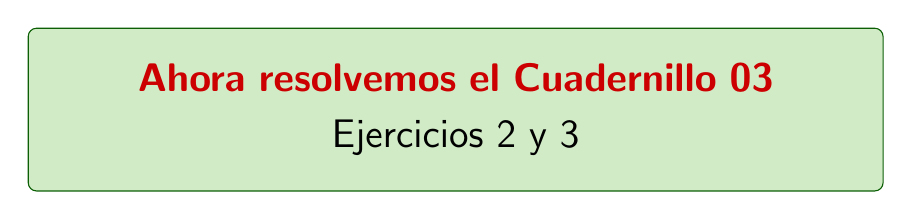
\begin{tikzpicture}
\node[idea,fill=pastelgreen,text width=.82\textwidth,inner sep=13pt,font=\Large]
{\actividad{Ahora resolvemos el Cuadernillo 03}\\[2pt]
Ejercicios 2 y 3};
\end{tikzpicture}
\end{center}

\bigskip
\begin{itemize}
\item \textbf{Ejercicio 2:} clasificar lexemas con los patrones aprobados de \texttt{LOC} y \texttt{NUM}.
\item \textbf{Ejercicio 3:} encontrar un contraejemplo que haga visible el error de cada propuesta.
\end{itemize}

\vfill
\end{frame}

\begin{frame}{AFN y AFD: mismo poder, distinto recorrido}
\vfill

\begin{center}
\small
\renewcommand{\arraystretch}{1.25}
\begin{tabular}{|L{.25\textwidth}|L{.29\textwidth}|L{.32\textwidth}|}
\hline
\textbf{Aspecto} & \textbf{AFN} & \textbf{AFD} \tabularnewline
\hline
Siguiente estado & Puede ser un conjunto de estados. & Es un solo estado. \tabularnewline
\hline
Transiciones \(\varepsilon\) & Se permiten. & No se permiten. \tabularnewline
\hline
Aceptación & Basta un recorrido que acepte. & Se sigue el único recorrido. \tabularnewline
\hline
Uso & Facilita componer subexpresiones. & Facilita reconocer símbolo por símbolo. \tabularnewline
\hline
\end{tabular}
\end{center}

\bigskip
\begin{block}{Equivalencia expresiva}
Para cada AFN existe un AFD que reconoce el mismo lenguaje.
\end{block}

\vfill
\end{frame}

\begin{frame}{Ejemplo resuelto: AFD para \texttt{NUM}}
\vfill

\begin{center}
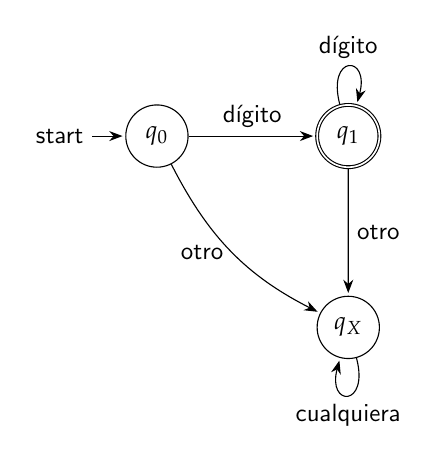
\begin{tikzpicture}[shorten >=1pt,node distance=2.7cm,on grid,auto,>=Stealth,scale=.90,transform shape]
\node[state,initial] (q0) {\(q_0\)};
\node[state,accepting,right=of q0] (q1) {\(q_1\)};
\node[state,below=of q1] (qx) {\(q_X\)};
\path[->]
  (q0) edge node {dígito} (q1)
       edge[bend right=18] node[left] {otro} (qx)
  (q1) edge[loop above] node {dígito} ()
       edge node[right] {otro} (qx)
  (qx) edge[loop below] node {cualquiera} ();
\end{tikzpicture}
\end{center}

\bigskip
\begin{columns}[T,onlytextwidth]
\begin{column}{.48\textwidth}
\begin{block}{Entrada \texttt{25}}
\centering \(q_0\to q_1\to q_1\): acepta.
\end{block}
\end{column}
\begin{column}{.48\textwidth}
\begin{block}{Entrada \texttt{2x}}
\centering \(q_0\to q_1\to q_X\): rechaza.
\end{block}
\end{column}
\end{columns}

\vfill
\end{frame}

\begin{frame}{Trabajo con el cuadernillo}
\vfill

\begin{center}
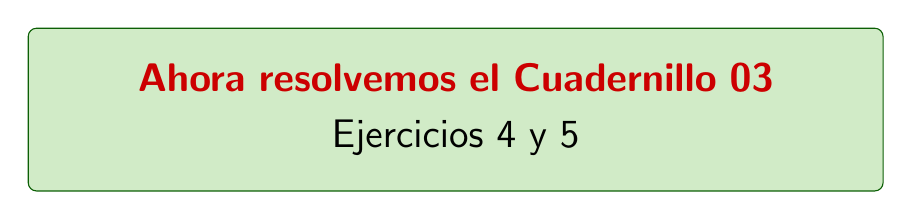
\begin{tikzpicture}
\node[idea,fill=pastelgreen,text width=.82\textwidth,inner sep=13pt,font=\Large]
{\actividad{Ahora resolvemos el Cuadernillo 03}\\[2pt]
Ejercicios 4 y 5};
\end{tikzpicture}
\end{center}

\bigskip
\begin{itemize}
\item \textbf{Ejercicio 4:} distinguir el funcionamiento de un AFN y un AFD.
\item \textbf{Ejercicio 5:} construir un AFD para \texttt{LOC} y trazar cuatro cadenas.
\end{itemize}

\vfill
\end{frame}

\begin{frame}{De una expresión regular a un AFN}
\vfill

\begin{block}{Método de Thompson}
Construye un AFN para cada subexpresión y combina las piezas siguiendo la estructura de la expresión regular.
\end{block}

\bigskip

\begin{center}
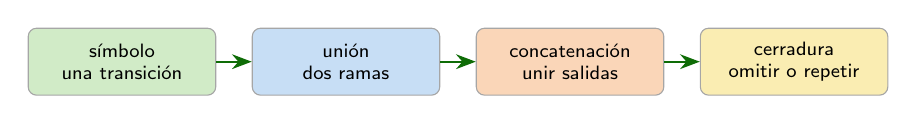
\begin{tikzpicture}[node distance=.45cm]
\node[mini,fill=pastelgreen,text width=2.1cm] (a) {símbolo\\una transición};
\node[mini,fill=pastelblue,right=of a,text width=2.1cm] (b) {unión\\dos ramas};
\node[mini,fill=pastelpeach,right=of b,text width=2.1cm] (c) {concatenación\\unir salidas};
\node[mini,fill=pastelyellow,right=of c,text width=2.1cm] (d) {cerradura\\omitir o repetir};
\draw[arrow] (a) -- (b);
\draw[arrow] (b) -- (c);
\draw[arrow] (c) -- (d);
\end{tikzpicture}
\end{center}

\bigskip
\begin{center}
\small Las transiciones \(\varepsilon\) permiten conectar componentes sin consumir entrada.
\end{center}

\vfill
\end{frame}

\begin{frame}{Ejemplo resuelto: AFN de Thompson para \(a\mid b\)}
\vfill

\begin{center}
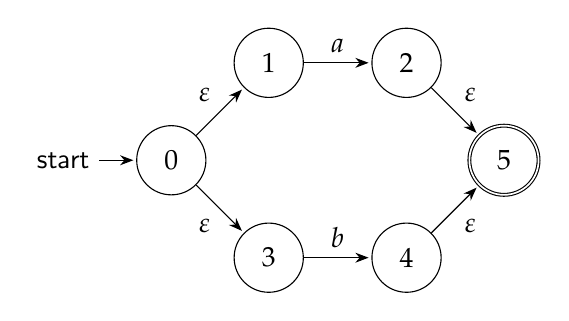
\begin{tikzpicture}[shorten >=1pt,node distance=1.75cm,on grid,auto,>=Stealth]
\node[state,initial] (q0) {\(0\)};
\node[state,above right=of q0] (q1) {\(1\)};
\node[state,right=of q1] (q2) {\(2\)};
\node[state,below right=of q0] (q3) {\(3\)};
\node[state,right=of q3] (q4) {\(4\)};
\node[state,accepting,below right=of q2] (q5) {\(5\)};
\path[->]
  (q0) edge node[above left] {\(\varepsilon\)} (q1)
       edge node[below left] {\(\varepsilon\)} (q3)
  (q1) edge node {\(a\)} (q2)
  (q3) edge node {\(b\)} (q4)
  (q2) edge node[above right] {\(\varepsilon\)} (q5)
  (q4) edge node[below right] {\(\varepsilon\)} (q5);
\end{tikzpicture}
\end{center}

\bigskip
\begin{itemize}
\item \(a\): \(0\xrightarrow{\varepsilon}1\xrightarrow{a}2\xrightarrow{\varepsilon}5\); acepta.
\item \(b\): sigue la rama inferior y acepta.
\item \(ab\): ninguna rama consume toda la entrada; rechaza.
\end{itemize}

\vfill
\end{frame}

\begin{frame}{Construcción de subconjuntos}
\vfill

\begin{block}{Dos operaciones}
\small
\term{cerradura-\(\varepsilon\)} reúne los estados alcanzables sin consumir símbolos.\par
\term{mover\((T,a)\)} reúne los estados alcanzables desde \(T\) al consumir \(a\).
\end{block}

\bigskip
\begin{enumerate}
\item Inicia con \(A_0=\operatorname{cerradura}_{\varepsilon}(\{q_0\})\).
\item Para cada conjunto \(T\) y símbolo \(a\), calcula
\[
U=\operatorname{cerradura}_{\varepsilon}(\operatorname{mover}(T,a)).
\]
\item Agrega \(U\) sólo si todavía no se había descubierto.
\item Marca \(U\) como aceptación cuando \(U\cap F\neq\emptyset\).
\item Repite hasta que no queden conjuntos pendientes.
\end{enumerate}

\vfill
\end{frame}

\begin{frame}{El AFN de \(a\mid b\) convertido a AFD}
\vfill

\[
\begin{aligned}
A&=\{0,1,3\}, &
B&=\{2,5\},\\
C&=\{4,5\}, &
D&=\emptyset.
\end{aligned}
\]

\begin{center}
\small
\renewcommand{\arraystretch}{1.2}
\begin{tabular}{|c|c|c|c|}
\hline
\textbf{Estado} & \textbf{Con \(a\)} & \textbf{Con \(b\)} & \textbf{Acepta} \tabularnewline
\hline
\(A\) & \(B\) & \(C\) & No \tabularnewline
\hline
\(B\) & \(D\) & \(D\) & Sí \tabularnewline
\hline
\(C\) & \(D\) & \(D\) & Sí \tabularnewline
\hline
\(D\) & \(D\) & \(D\) & No \tabularnewline
\hline
\end{tabular}
\end{center}

\bigskip
\begin{center}
\term{Un estado del AFD representa un conjunto de estados posibles del AFN.}
\end{center}

\vfill
\end{frame}

\begin{frame}{Trabajo con el cuadernillo}
\vfill

\begin{center}
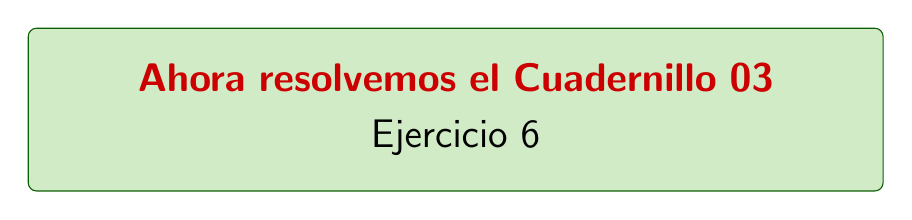
\begin{tikzpicture}
\node[idea,fill=pastelgreen,text width=.82\textwidth,inner sep=13pt,font=\Large]
{\actividad{Ahora resolvemos el Cuadernillo 03}\\[2pt]
Ejercicio 6};
\end{tikzpicture}
\end{center}

\bigskip
\begin{itemize}
\item Calcula las cerraduras y movimientos del AFN de \(a\mid b\).
\item Completa la tabla del AFD y marca los conjuntos de aceptación.
\item Compara los \(2^6=64\) subconjuntos posibles con los cuatro alcanzables.
\end{itemize}

\vfill
\end{frame}

\begin{frame}{Construimos sólo los subconjuntos alcanzables}
\vfill

\begin{center}
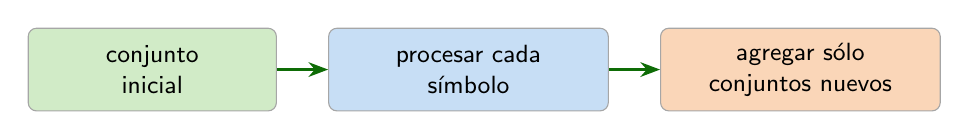
\begin{tikzpicture}[node distance=.65cm]
\node[bloque,fill=pastelgreen,text width=2.8cm] (a) {conjunto\\inicial};
\node[bloque,fill=pastelblue,right=of a,text width=3.2cm] (b) {procesar cada\\símbolo};
\node[bloque,fill=pastelpeach,right=of b,text width=3.2cm] (c) {agregar sólo\\conjuntos nuevos};
\draw[arrow] (a) -- (b);
\draw[arrow] (b) -- (c);
\end{tikzpicture}
\end{center}

\bigskip
\begin{block}{Conjunto potencia y estados efectivos}
Si el AFN tiene \(n\) estados, \(\mathcal{P}(Q)\) contiene hasta \(2^n\) subconjuntos. El AFD sólo necesita los que pueden alcanzarse desde su estado inicial.
\end{block}

\bigskip
\begin{center}
\small Cada conjunto se procesa una vez; el procedimiento termina cuando no aparecen estados nuevos.
\end{center}

\vfill
\end{frame}

\begin{frame}{Trabajo con el cuadernillo}
\vfill

\begin{center}
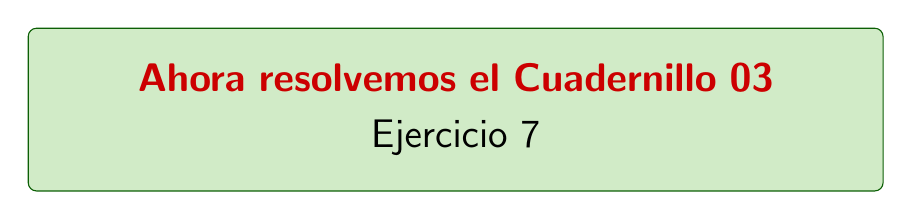
\begin{tikzpicture}
\node[idea,fill=pastelgreen,text width=.82\textwidth,inner sep=13pt,font=\Large]
{\actividad{Ahora resolvemos el Cuadernillo 03}\\[2pt]
Ejercicio 7};
\end{tikzpicture}
\end{center}

\bigskip
\begin{itemize}
\item Aplica la construcción a un AFN sin transiciones \(\varepsilon\).
\item Agrega únicamente los subconjuntos alcanzables.
\item Traza \texttt{1101} y describe el lenguaje reconocido.
\end{itemize}

\vfill
\end{frame}

\begin{frame}{Minimizar sin cambiar el lenguaje}
\vfill

\begin{columns}[T,onlytextwidth]
\begin{column}{.48\textwidth}
\begin{block}{Estados distinguibles}
\small Existe una continuación que, al comenzar en ambos estados, termina en aceptación sólo desde uno.
\end{block}
\end{column}
\begin{column}{.48\textwidth}
\begin{block}{Estados equivalentes}
\small Ninguna continuación permite distinguirlos; pueden reunirse en el AFD mínimo.
\end{block}
\end{column}
\end{columns}

\bigskip
\begin{enumerate}
\item Separa estados de aceptación y de no aceptación.
\item Dentro de cada grupo, compara a qué grupos llegan las transiciones.
\item Separa los estados cuyo comportamiento difiere.
\item Repite hasta obtener una partición estable.
\end{enumerate}

\vfill
\end{frame}

\begin{frame}{Ejemplo resuelto: minimizar el AFD de \(a\mid b\)}
\vfill

\[
\Pi_0=\big\{\{B,C\},\{A,D\}\big\}
\]

\begin{itemize}
\item \(B\) y \(C\) aceptan y, con \(a\) o \(b\), llegan a \(D\): permanecen juntos.
\item \(A\) y \(D\) se distinguen con \(a\): desde \(A\) se acepta y desde \(D\) no.
\end{itemize}

\[
\Pi_f=\big\{\{B,C\},\{A\},\{D\}\big\}
\]

\begin{center}
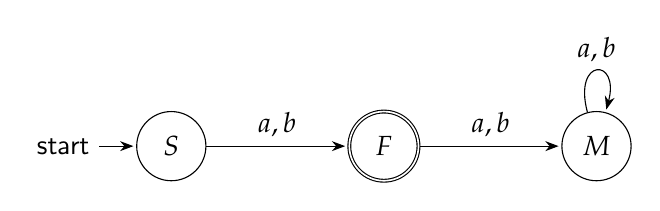
\begin{tikzpicture}[shorten >=1pt,node distance=2.7cm,on grid,auto,>=Stealth]
\node[state,initial] (S) {\(S\)};
\node[state,accepting,right=of S] (F) {\(F\)};
\node[state,right=of F] (M) {\(M\)};
\path[->]
  (S) edge node {\(a,b\)} (F)
  (F) edge node {\(a,b\)} (M)
  (M) edge[loop above] node {\(a,b\)} ();
\end{tikzpicture}
\end{center}

\vfill
\end{frame}

\begin{frame}{Trabajo con el cuadernillo}
\vfill

\begin{center}
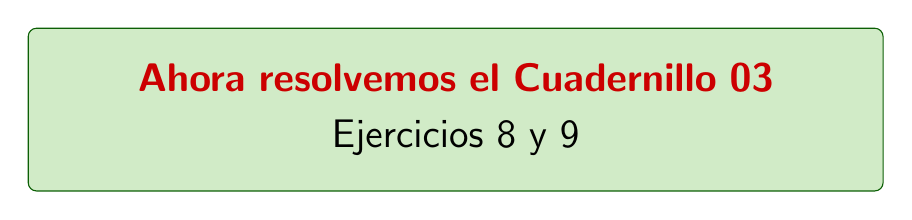
\begin{tikzpicture}
\node[idea,fill=pastelgreen,text width=.82\textwidth,inner sep=13pt,font=\Large]
{\actividad{Ahora resolvemos el Cuadernillo 03}\\[2pt]
Ejercicios 8 y 9};
\end{tikzpicture}
\end{center}

\bigskip
\begin{itemize}
\item \textbf{Ejercicio 8:} aplicar la tabla de pares al AFD de \(a\mid b\).
\item \textbf{Ejercicio 9:} refinar una partición hasta construir otro AFD mínimo.
\end{itemize}

\vfill
\end{frame}

\begin{frame}{Aplicación integrada a un fragmento de IMP}
\vfill

\begin{block}{Entrada}
\centering
\texttt{if x20 <= 25 then x20 := x20 + 1 else skip}
\end{block}

\bigskip
\begin{center}
\scriptsize
\renewcommand{\arraystretch}{1.18}
\begin{tabular}{|c|c|L{.43\textwidth}|}
\hline
\textbf{Lexema} & \textbf{Token} & \textbf{Patrón o lexema fijo} \tabularnewline
\hline
\texttt{if} & \texttt{IF} & Lexema fijo \texttt{if}. \tabularnewline
\hline
\texttt{x20} & \texttt{LOC(x20)} & \(\mathit{letra}^{+}\mathit{digito}^{*}\). \tabularnewline
\hline
\texttt{<=} & \texttt{LE} & Lexema fijo \texttt{<=}. \tabularnewline
\hline
\texttt{25} & \texttt{NUM(25)} & \(\mathit{digito}^{+}\). \tabularnewline
\hline
\texttt{:=} & \texttt{ASSIGN} & Lexema fijo \texttt{:=}. \tabularnewline
\hline
\texttt{+} & \texttt{PLUS} & Lexema fijo \texttt{+}. \tabularnewline
\hline
\end{tabular}
\end{center}

\bigskip
\begin{center}
\scriptsize \texttt{IF LOC(x20) LE NUM(25) THEN LOC(x20) ASSIGN LOC(x20) PLUS NUM(1) ELSE SKIP}
\end{center}

\vfill
\end{frame}

\begin{frame}{Qué hemos construido y qué falta}
\vfill

\begin{center}
\resizebox{.96\textwidth}{!}{%
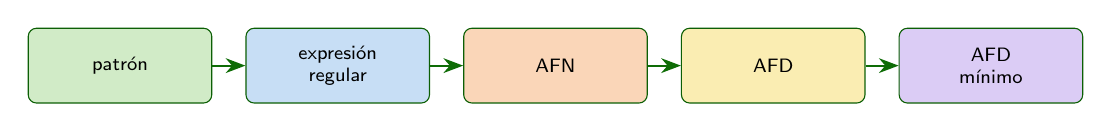
\begin{tikzpicture}[node distance=.42cm]
\node[paso,fill=pastelgreen,text width=2.05cm] (a) {patrón};
\node[paso,fill=pastelblue,right=of a,text width=2.05cm] (b) {expresión\\regular};
\node[paso,fill=pastelpeach,right=of b,text width=2.05cm] (c) {AFN};
\node[paso,fill=pastelyellow,right=of c,text width=2.05cm] (d) {AFD};
\node[paso,fill=pastelviolet,right=of d,text width=2.05cm] (e) {AFD\\mínimo};
\draw[arrow] (a) -- (b);
\draw[arrow] (b) -- (c);
\draw[arrow] (c) -- (d);
\draw[arrow] (d) -- (e);
\end{tikzpicture}%
}
\end{center}

\bigskip
\begin{block}{En el tema 2.3 todavía falta}
\small
\begin{itemize}
\item coordinar todas las reglas y resolver coincidencias;
\item identificar el lexema adecuado dentro del flujo;
\item omitir los espacios permitidos y reportar errores;
\item expresar la especificación en \textsc{Lark}.
\end{itemize}
\end{block}

\vfill
\end{frame}

\begin{frame}{Trabajo con el cuadernillo}
\vfill

\begin{center}
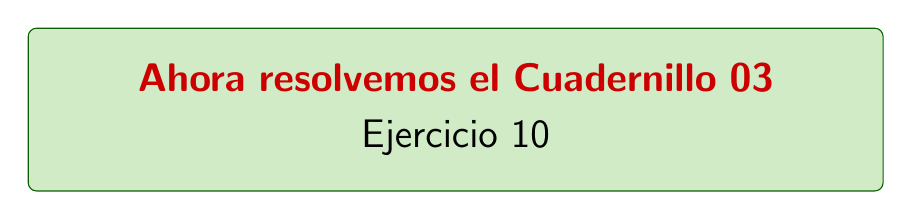
\begin{tikzpicture}
\node[idea,fill=pastelgreen,text width=.82\textwidth,inner sep=13pt,font=\Large]
{\actividad{Ahora resolvemos el Cuadernillo 03}\\[2pt]
Ejercicio 10};
\end{tikzpicture}
\end{center}

\bigskip
\begin{itemize}
\item Separa los lexemas y escribe la secuencia conceptual de tokens.
\item Relaciona \texttt{x20} y \texttt{25} con sus patrones.
\item Ordena la ruta del patrón al AFD mínimo.
\item Delimita el trabajo que corresponde al tema 2.3.
\end{itemize}

\vfill
\end{frame}

\begin{frame}{Confusiones que debemos evitar}
\vfill

\begin{center}
\scriptsize
\renewcommand{\arraystretch}{1.23}
\begin{tabular}{|L{.39\textwidth}|L{.47\textwidth}|}
\hline
\textbf{Confusión} & \textbf{Corrección} \tabularnewline
\hline
Una expresión regular es una cadena de ejemplo. & La expresión describe un lenguaje; una cadena puede pertenecer o no a él. \tabularnewline
\hline
Un AFN acepta sólo si todos sus recorridos aceptan. & Basta que exista un recorrido que consuma toda la entrada y acepte. \tabularnewline
\hline
Una transición \(\varepsilon\) consume un símbolo. & Cambia de estado sin consumir entrada. \tabularnewline
\hline
Todo subconjunto posible aparece en el AFD. & Sólo se incorporan los subconjuntos alcanzables desde el inicio. \tabularnewline
\hline
Minimizar puede cambiar las cadenas aceptadas. & El AFD mínimo debe reconocer exactamente el mismo lenguaje. \tabularnewline
\hline
\end{tabular}
\end{center}

\vfill
\end{frame}

\begin{frame}{Conclusión}
\vfill

\begin{center}
\resizebox{.96\textwidth}{!}{%
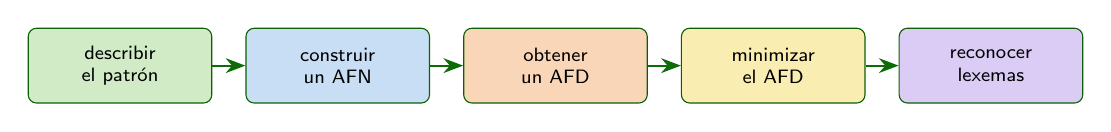
\begin{tikzpicture}[node distance=.42cm]
\node[paso,fill=pastelgreen,text width=2.05cm] (a) {describir\\el patrón};
\node[paso,fill=pastelblue,right=of a,text width=2.05cm] (b) {construir\\un AFN};
\node[paso,fill=pastelpeach,right=of b,text width=2.05cm] (c) {obtener\\un AFD};
\node[paso,fill=pastelyellow,right=of c,text width=2.05cm] (d) {minimizar\\el AFD};
\node[paso,fill=pastelviolet,right=of d,text width=2.05cm] (e) {reconocer\\lexemas};
\draw[arrow] (a) -- (b);
\draw[arrow] (b) -- (c);
\draw[arrow] (c) -- (d);
\draw[arrow] (d) -- (e);
\end{tikzpicture}%
}
\end{center}

\bigskip
\begin{block}{Idea de cierre}
Las expresiones regulares especifican los lenguajes de los tokens y los autómatas permiten reconocer sus cadenas. Thompson, la construcción de subconjuntos y la minimización cambian la representación sin cambiar el lenguaje.
\end{block}

\bigskip
\begin{center}
\term{Ya contamos con la base formal para construir el analizador léxico de IMP.}
\end{center}

\vfill
\end{frame}

\begin{frame}{Referencias}
\vfill

\tiny
\begin{enumerate}
\item Soto Romero, M. y Reyes Cabello, A. L. (2026). \textit{Programación de Sistemas. Nota de clase 04: Expresiones regulares y autómatas finitos}. Colegio de Ciencia y Tecnología, UACM.
\item Soto Romero, M. y Reyes Cabello, A. L. (2026). \textit{Programación de Sistemas. Cuadernillo de ejercicios 03: Expresiones regulares y autómatas}. Colegio de Ciencia y Tecnología, UACM.
\item Aho, A. V., Lam, M. S., Sethi, R., y Ullman, J. D. (2006). \textit{Compilers: Principles, techniques, and tools} (2nd ed.). Pearson.
\item Vilar Torres, J. M. (2010). \textit{Analizador léxico}. Universitat Jaume I.
\item Soto Romero, M. (2021). \textit{Autómatas finitos} (Nota de clase 3, Teoría de la Computación). Colegio de Ciencia y Tecnología, UACM.
\item Soto Romero, M. (2021). \textit{Autómatas finitos con \(\varepsilon\)-transiciones} (Nota de clase 5, Teoría de la Computación). Colegio de Ciencia y Tecnología, UACM.
\end{enumerate}

\vfill
\end{frame}

\end{document}
